We now want to rewrite the linear and non-linear HOPS equations (\ref{eq:linear_HOPS_single_site}, \ref{eq:non_linear_HOPS_single_site}) 
in such a way that we can use them together with the MPS formalism. We will do the derivation for the non-linear
equation, following reference \cite{Gao:2022}. The linear equation can be derived analogeously.
\\
We start by representing the full hierarchy at time $t$ by a single quantum state
\begin{equation}
    \label{eq:full_HOPS_state_non_mps}
        \ket*{\vb*{\Psi_t}} = \sum_{l, \vb{n}} \Psi_t^{l,(\vb{n})} \ket*{l, n_1, n_2, \dots, n_{K}}.
\end{equation}
The HOPS equations then become
\begin{equation*}
    \frac{\partial}{\partial t}\Psi_t^{l,(\vb{n})} = \left(
        -i\hat{H}_\text{S} - \vectorbold{n}\cdot\boldsymbol{\omega} + \hat{L}\tilde{z}_t^*
    \right) \Psi_t^{l,(\vb{n})}
    + L\sum_{k=1}^{K}n_kg_k\Psi_t^{l,(\vb{n}-\vb*{e}_k)}
    - \left(
        \hat{L}^\dagger - \langle
        \hat{L}^\dagger
    \rangle_t
    \right)\sum_{k=1}^{K}\Psi_t^{l,(\vb{n}+\vb*{e}_k)},
\end{equation*}
where $\vb{e}_k$ again denotes the $k$th unit vector. Next, we define the ladder operators
\begin{equation*}
    \begin{split}
        \hat{b}_k^\dagger \ket*{\vb{n}} &\coloneqq \ket*{\vb{n} + \vb{e}_k} \\
        \hat{b}_k \ket*{\vb{n}} &\coloneqq \ket*{\vb{n} - \vb{e}_k}
    \end{split}
\end{equation*}
and the number operator
\begin{equation*}
    \hat{N}_k \ket*{\vb{n}} \coloneqq n_k \ket*{\vb{n}}
\end{equation*}
and use them to write an update equation for the full state:
\begin{equation*}
    \frac{\partial}{\partial t}\ket*{\vb*{\Psi_t}} = -i\hat{H}_\text{eff} \ket*{\vb*{\Psi_t}},
\end{equation*}
with the effective Hamiltonian
\begin{equation}
    \label{eq:effective_HOPS_Hamiltonian_multiple_bath_modes}
    \begin{split}
        \hat{H}_\text{eff} = \,\,&\hat{H}_\text{S} \otimes \mathbb{1} - i\sum_{k=1}^{K} \omega_k \cdot \mathbb{1} \otimes \hat{N}_k + i\tilde{z}_t^*\cdot\hat{L} \otimes \mathbb{1}\\
        &+ i\sum_{k=1}^{K} g_k \cdot \hat{L} \otimes \hat{N}_k\hat{b}^\dagger_k - i\sum_{k=1}^{K} \left(\hat{L}^\dagger - \langle\hat{L}^\dagger\rangle_t\right) \otimes \hat{b}_k.
    \end{split}
\end{equation}
Finally, we can now go to the MPS formalism. We can write the full state (\ref{eq:full_HOPS_state_non_mps}) as an MPS
\begin{equation*}
    \ket*{\vb*{\Psi_t}} = \sum_{l,\vb{n},\vb{a}} A_{a_0, a_1}^{[1], l} A_{a_1, a_2}^{[2], n_1} A_{a_2, a_3}^{[3], n_2} \cdots A_{a_K, a_0}^{[K+1] n_K} \ket*{l, n_1, n_2, \dots, n_{K}},
\end{equation*}
using $K+1$ tensors in total. The last thing we still need to do is to write the effective Hamiltonian (\ref{eq:effective_HOPS_Hamiltonian_multiple_bath_modes})
in MPO form. This can for example be done by using the finite state machine method discussed in \cite{Motruk:2016}. By using the finite state machine depicted
in figure \ref{}, we arrive at the following tensors:
\begin{equation}
    \label{eq:HOMPS_MPO}
    \begin{aligned}
        \vb*{W^{[1]}} \coloneqq
        \begin{pmatrix}
            -i\mathbb{1} & i\hat{L} & i\left(\left\langle \hat{L}^\dagger\right\rangle \mathbb{1} - \hat{L}^\dagger\right) & \hat{H}_\text{S} + i\tilde{z}_t^*\hat{L} \\
            0            & 0        & 0                                                                                    & 0                                        \\
            0            & 0        & 0                                                                                    & 0                                        \\
            0            & 0        & 0                                                                                    & 0                                        \\
        \end{pmatrix},\\
        \vb*{W^{[k+1]}} \coloneqq
        \begin{pmatrix}
            \mathbb{1} & 0          & 0          & \omega_k\hat{N}_k                \\
            0          & \mathbb{1} & 0          & g_k \hat{N}_k  \hat{b}_k^\dagger \\
            0          & 0          & \mathbb{1} & \hat{b}_k                        \\
            0          & 0          & 0          & \mathbb{1}                       \\
        \end{pmatrix}, \quad k = 1, 2, \dots, K.
    \end{aligned}
\end{equation}
\begin{figure}
    \centering
    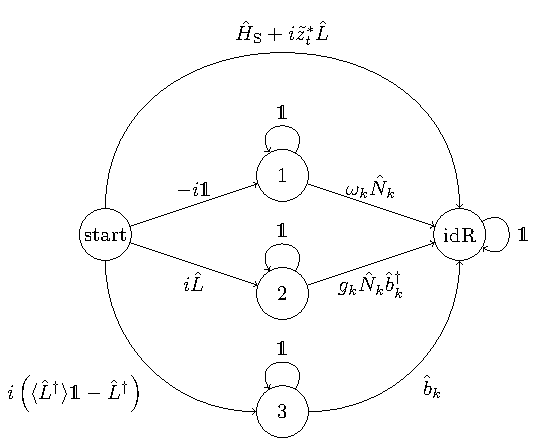
\includegraphics{figures/tikz/state_machine/state_machine.pdf}
    \caption{In this figure the state machine that can be used to generate the MPO (\ref{eq:HOMPS_MPO}) is sketched.
    The state machine can be constructed from equation (\ref{eq:effective_HOPS_Hamiltonian_multiple_bath_modes}). For
    reference on how to use state machines to construct MPOs, see \cite{Motruk:2016}}
    \label{fig:state_machine}
\end{figure}